\chapter{实验设计与结果分析}
\label{chap:experiment}

本章通过系统性的实验验证本文提出的基于驱动程序替换的固件仿真方法的有效性。实验从多个维度对方法进行评估，包括静态分析模块的识别与替换能力、运行正确性、方法对比以及应用验证。

\section{实验设计}
\label{sec:design}

为了全面评估本文方法的有效性和实用性，本节介绍实验的整体设计，包括实验环境的搭建、测试用例的选择以及实验目标的定义。

\subsection{实验环境}

实验在以下软硬件环境中进行，具体配置如表~\ref{tab:hw_env}和表~\ref{tab:sw_env}所示。两表分别给出硬件资源与软件栈信息，便于后续效率与可复现性分析。

\begin{table}[htbp]
\centering
\caption{硬件环境配置}
\label{tab:hw_env}
\footnotesize
\begin{tabular}{ll}
\toprule
\textbf{配置项} & \textbf{规格} \\
\midrule
主机 & Intel Xeon Platinum 8350C 处理器（128核心），503GB 内存，869GB SSD \\
\bottomrule
\end{tabular}
\end{table}

\begin{table}[htbp]
\centering
\caption{软件环境配置}
\label{tab:sw_env}
\footnotesize
\begin{tabular}{ll}
\toprule
\textbf{配置项} & \textbf{规格} \\
\midrule
操作系统 & Ubuntu 22.04 LTS \\
编译工具链 & ARM GCC 10.3.1、CMake 3.21.4 \\
仿真环境 & Unicorn 2.0.2、UnicornAFL（基于Unicorn的模糊测试扩展） \\
模糊测试 & AFL++ 4.08c+（基于v4.08c的开发版本） \\
大模型 & DeepSeek V3.2 \\
\bottomrule
\end{tabular}
\end{table}

\subsection{测试用例}

为了验证方法的通用性和有效性，本研究构建了涵盖不同芯片平台、操作系统、驱动复杂度和外设类型的固件测试集。需要说明的是，受限于闭源商用固件的可获取性和法律合规要求，本研究的测试固件均来源于公开渠道，包括芯片厂商官方SDK示例和开源社区项目。

\textbf{（1）芯片平台选择}

测试固件覆盖了物联网设备中常见的三类主流 MCU 平台：STM32 系列（ARM Cortex-M4/M7）、NXP i.MX RT 系列（ARM Cortex-M7）和 Atmel SAM 系列（ARM Cortex-M4/M7）。

\textbf{（2）操作系统选择}

测试固件覆盖了四种典型的嵌入式软件架构：FreeRTOS、RT-Thread、Zephyr 和裸机。FreeRTOS 是全球使用最广泛的开源实时操作系统，具有内核精简、易于移植的特点，支持任务管理、队列、信号量等功能。RT-Thread 是国产开源实时操作系统，提供完整的设备驱动框架和丰富的软件包生态，在国内物联网领域应用广泛。Zephyr 是 Linux 基金会主导的开源实时操作系统，面向资源受限的物联网设备，提供统一的设备驱动模型和丰富的外设支持，近年来在工业和消费级 IoT 领域快速普及。裸机是指无操作系统支持的固件，所有驱动和应用代码直接运行在硬件上，常见于资源极度受限的物联网设备。

\textbf{（3）外设类型选择}

测试固件涵盖了物联网设备中常见的三类外设驱动，详细信息如表~\ref{tab:peripherals}所示。该分类用于后续按外设类型开展分组统计与对比分析。

\begin{table}[htbp]
\centering
\caption{外设类型分类}
\label{tab:peripherals}
\begin{adjustbox}{max width=\textwidth}
\begin{tabular}{ll}
\toprule
\textbf{类别} & \textbf{外设类型} \\
\midrule
通信外设 & UART（串口通信）、I2C（总线通信）、SPI（串行外设接口）、ETH（以太网控制器） \\
存储外设 & Flash（闪存控制器）、SDIO（SD卡接口） \\
定时器外设 & TIM（通用定时器）、RTC（实时时钟）、WDT（看门狗定时器） \\
\bottomrule
\end{tabular}
\end{adjustbox}
\end{table}

\textbf{（4）测试固件构建}

本研究测试固件来源于三类公开渠道：一是从 STM32CubeMX 和 NXP MCUXpresso SDK 提取的官方示例程序，这类程序代表规范的驱动代码编写风格，驱动接口清晰、结构标准化，适合验证方法的基本有效性；二是从 GitHub 和 Gitee 收集的开源物联网设备项目，如 RT-Thread 的板级支持包（BSP）和社区贡献的应用项目，这类项目代码规模更大、驱动逻辑更复杂；三是 Zephyr 项目的官方示例程序和板级支持包，Zephyr 采用统一的设备驱动模型（DM），其驱动代码风格与 FreeRTOS/RT-Thread 的 HAL 驱动存在显著差异，能够验证方法对不同驱动框架的通用性。需要指出的是，本测试集未包含闭源商用固件，对代码混淆、固件加密等对抗性场景尚未涉及，方法在真实商用固件上的适用性有待进一步验证。

经过筛选和整理，最终构建了包含 35 个固件的测试集，详细信息如表~\ref{tab:firmware}所示。该测试集覆盖不同平台、系统与外设组合，用于验证方法的通用性。

\begin{table}[H]
\centering
% 模板 \@makecaption 默认标题上下各 12bp；本表等高 minipage+resizebox 易再叠一行距，此处仅收紧本表
\begingroup
\setlength{\abovecaptionskip}{6bp}%
\setlength{\belowcaptionskip}{2bp}%
\caption{测试固件详细信息}%
\label{tab:firmware}%
\endgroup
\vspace{-0.65\baselineskip}%
% 先测两侧高度取 max，等高 minipage 顶对齐 +\vfill 兜底底边对齐；右表较矮，在末行前补一行空行（约一行差）
\begingroup
\setlength{\tabcolsep}{2pt}%
\setbox0=\hbox{\footnotesize\begin{tabular}[t]{lllll}
\toprule
\textbf{平台} & \textbf{OS} & \textbf{测试用例名称} & \textbf{MCU} & \textbf{外设} \\
\midrule
\multirow{6}{*}{STM32} & \multirow{6}{*}{RT-Thread} & stm32f401/base & F401 & 多外设 \\
 & & stm32f401/eth & F401 & ETH \\
 & & stm32f401/fatfs & F401 & SD \\
 & & stm32f401/fatfs\_sdcard & F401 & SD \\
 & & stm32f401/i2c & F401 & I2C \\
 & & stm32f401/uart & F401 & UART \\
\midrule
\multirow{4}{*}{STM32} & \multirow{4}{*}{FreeRTOS} & HTTP\_Server\_SockRT & STM32 & ETH \\
 & & HTTP\_Server\_Sock\_RT & STM32 & ETH \\
 & & LwIP\_StreamingSrv & STM32 & ETH \\
 & & UART\_Hyperterminal & STM32 & UART \\
\midrule
\multirow{4}{*}{STM32} & \multirow{4}{*}{Zephyr} & eth\_dhcpv4\_f767zi & F767ZI & ETH \\
 & & fs\_littlefs\_l475 & L475 & Flash \\
 & & i2c\_hts221\_l475 & L475 & I2C \\
 & & uart\_echo\_l475 & L475 & UART \\
\midrule
\multirow{4}{*}{Atmel} & \multirow{4}{*}{Zephyr} & eth\_dhcpv4\_e70 & SAM E70 & ETH \\
 & & fs\_littlefs\_same54 & ATSAME54 & Flash \\
 & & i2c\_shell\_same54 & ATSAME54 & I2C \\
 & & uart\_echo\_same54 & ATSAME54 & UART \\
\bottomrule
\end{tabular}}%
\setbox2=\hbox{\footnotesize\begin{tabular}[t]{lllll}
\toprule
\textbf{平台} & \textbf{OS} & \textbf{测试用例名称} & \textbf{MCU} & \textbf{外设} \\
\midrule
\multirow{4}{*}{NXP} & \multirow{4}{*}{裸机} & FATFS\_BareMetal & RT1052 & SD \\
 & & I2C\_BareMetal & RT1052 & I2C \\
 & & LwIP\_BareMetal & RT1052 & ETH \\
 & & UART\_BareMetal & RT1052 & UART \\
\midrule
\multirow{3}{*}{NXP} & \multirow{3}{*}{FreeRTOS} & FATFS\_FreeRTOS & RT1052 & SD \\
 & & LwIP\_FreeRTOS & RT1052 & ETH \\
 & & UART\_FreeRTOS & RT1052 & UART \\
\midrule
\multirow{6}{*}{NXP} & \multirow{6}{*}{RT-Thread} & imxrt1052/base & RT1052 & 多外设 \\
 & & imxrt1052/fatfs & RT1052 & SD \\
 & & imxrt1052/i2c & RT1052 & I2C \\
 & & imxrt1052/uart & RT1052 & UART \\
 & & imxrt1060/base & RT1060 & 多外设 \\
 & & imxrt1060/eth & RT1060 & ETH \\
\midrule
\multirow{4}{*}{NXP} & \multirow{4}{*}{Zephyr} & eth\_dhcpv4\_rt1060 & RT1060 & ETH \\
 & & fs\_littlefs\_rt1060 & RT1060 & Flash \\
 & & i2c\_fxos8700\_lpc55 & LPC55S69 & I2C \\
 & & uart\_echo\_rt1060 & RT1060 & UART \\
 & & & & \\
\bottomrule
\end{tabular}}%
\dimen0=\dimexpr\ht0+\dp0\relax
\dimen2=\dimexpr\ht2+\dp2\relax
\ifdim\dimen2>\dimen0
  \dimen0=\dimen2
\fi
\resizebox{\textwidth}{!}{%
  \footnotesize
  \setlength{\tabcolsep}{2pt}%
  \begin{minipage}[t][\dimen0][t]{\wd0}%
  \vspace{0pt}\copy0\vfill
  \end{minipage}%
  \hspace{1.2em}%
  \begin{minipage}[t][\dimen0][t]{\wd2}%
  \vspace{0pt}\copy2\vfill
  \end{minipage}%
}%
\endgroup

\vspace{2pt}

{\scriptsize 共35个固件，覆盖NXP/STM32/Atmel三种平台，FreeRTOS/RT-Thread/Zephyr/裸机四种操作系统}
\end{table}

\section{驱动函数识别与替换统计}
\label{sec:driver_stats}

驱动函数识别与分类是整个替换流程的基础环节，分类准确性直接影响后续替换策略的选择和替换代码的质量。本节评估系统对驱动函数的自动识别与替换能力，验证静态分析模块的函数识别准确性和LLM的替换代码生成效果。

为了全面评估本文方法的驱动处理能力，本研究统计了每个测试用例的驱动函数识别和替换情况（完整分类统计数据见附录表~\ref{tab:function_categories_stats}）。表~\ref{tab:driver_stats}展示了各测试用例的驱动函数识别与替换统计。

\begin{table}[H]
\centering
\caption{驱动函数识别与替换统计}
\label{tab:driver_stats}
\footnotesize
\setlength{\tabcolsep}{2pt}
% 左栏末行总计、右栏末行平均，列与表头对齐；整块 resizebox 防超宽
\resizebox{\textwidth}{!}{%
\begin{tabular}{@{}c@{\hspace{0.55em}}c@{}}
\begin{tabular}[t]{lccc}
\toprule
\textbf{测试用例名称} & \textbf{识别数} & \textbf{替换数} & \textbf{迭代数} \\
\midrule
NXP\_FATFS\_BareMetal & 67 & 37 & 26 \\
NXP\_FATFS\_FreeRTOS & 65 & 36 & 34 \\
NXP\_I2C\_BareMetal & 104 & 50 & 45 \\
NXP\_LwIP\_BareMetal & 105 & 61 & 20 \\
NXP\_LwIP\_FreeRTOS & 107 & 70 & 9 \\
NXP\_UART\_BareMetal & 90 & 49 & 33 \\
NXP\_UART\_FreeRTOS & 91 & 39 & 25 \\
imxrt1052-nxp-evk/base & 53 & 34 & 18 \\
imxrt1052-nxp-evk/fatfs & 53 & 31 & 24 \\
imxrt1052-nxp-evk/i2c & 110 & 50 & 33 \\
imxrt1052-nxp-evk/uart & 73 & 41 & 20 \\
imxrt1060-nxp-evk/base & 65 & 5 & 4 \\
imxrt1060-nxp-evk/eth & 73 & 6 & 5 \\
stm32f401-st-nucleo/base & 55 & 32 & 26 \\
stm32f401-st-nucleo/eth & 55 & 35 & 19 \\
stm32f401-st-nucleo/fatfs & 56 & 40 & 14 \\
stm32f401-st-nucleo/fatfs\_sdcard & 281 & 161 & 18 \\
stm32f401-st-nucleo/i2c & 55 & 33 & 5 \\
\midrule
\textbf{总计} & \textbf{4029} & \textbf{1563} & \textbf{513} \\
\bottomrule
\end{tabular}
&
\begin{tabular}[t]{lccc}
\toprule
\textbf{测试用例名称} & \textbf{识别数} & \textbf{替换数} & \textbf{迭代数} \\
\midrule
stm32f401-st-nucleo/uart & 55 & 39 & 11 \\
LwIP\_HTTP\_Server\_SocketRTOS & 281 & 161 & 18 \\
LwIP\_HTTP\_Server\_Socket\_RTOS & 304 & 213 & 17 \\
LwIP\_StreamingServer & 281 & 161 & 18 \\
UART\_Hyperterminal\_IT & 120 & 87 & 8 \\
eth\_dhcpv4\_sam\_e70 & 188 & 12 & 7 \\
fs\_littlefs\_atsame54 & 76 & 19 & 25 \\
i2c\_shell\_atsame54 & 79 & 14 & 11 \\
uart\_echo\_atsame54 & 63 & 13 & 13 \\
eth\_dhcpv4\_mimxrt1060 & 276 & 12 & 5 \\
fs\_littlefs\_mimxrt1060 & 113 & 2 & 2 \\
i2c\_fxos8700\_lpc55 & 150 & 3 & 0 \\
uart\_echo\_mimxrt1060 & 103 & 2 & 0 \\
eth\_dhcpv4\_nucleo\_f767zi & 260 & 15 & 0 \\
fs\_littlefs\_disco\_l475 & 50 & 0 & 0 \\
i2c\_hts221\_disco\_l475 & 37 & 0 & 0 \\
uart\_echo\_disco\_l475 & 35 & 0 & 0 \\
 & & & \\
\midrule
\textbf{平均} & \textbf{115.1} & \textbf{44.7} & \textbf{14.7} \\
\bottomrule
\end{tabular}
\end{tabular}%
}%
\end{table}

从统计结果可以看出，本文方法在驱动函数识别和替换方面表现出较高的准确性。35个测试用例共识别出4029个驱动函数，平均每个固件115.1个；成功生成1563个替换代码，平均每个固件44.7个。其中513个替换代码经过动态反馈闭环进行了迭代优化，平均每个固件14.7个。替换代码生成率为38.8\%（1563/4029），未生成替换代码的函数主要包括两类：一是 NODRIVER 类纯业务逻辑函数（812个，占20.2\%），这类函数不直接访问硬件寄存器，无需替换；二是 PUREDRV 类简单驱动函数（978个，占24.3\%），该类由 RETURNOK 与 SKIP 合并而成，在仿真环境中可通过直接返回成功或保留最小语义路径运行，无需额外生成复杂替换代码。

% 本实验的主要目的包括：第一，验证本文方法能够准确识别固件中的硬件依赖代码；第二，验证本文方法生成的替代代码能够在仿真环境中正确执行，保证固件的正常运行；第三，验证本文方法对不同平台、不同操作系统、不同外设类型的固件具有通用性和可扩展性；第四，验证仿真环境能够支持模糊测试和漏洞挖掘任务。

\section{驱动函数分类统计}
\label{sec:classify_stats}

为了全面评估本文方法的驱动函数分类能力，本研究统计了每个测试用例的驱动函数按类别分布情况（完整统计数据见附录表~\ref{tab:function_categories_stats}）。图~\ref{fig:classification_pie}展示了各类驱动函数的占比分布情况。

\begin{figure}[htbp]
\centering
\definecolor{cINIT}{RGB}{70,130,195}
\definecolor{cNODRIVER}{RGB}{160,160,160}
\definecolor{cLOOP}{RGB}{235,165,65}
\definecolor{cPUREDRV}{RGB}{80,165,80}
\definecolor{cRECV}{RGB}{210,80,80}
\definecolor{cIRQ}{RGB}{230,190,60}
\definecolor{cCORE}{RGB}{150,100,180}
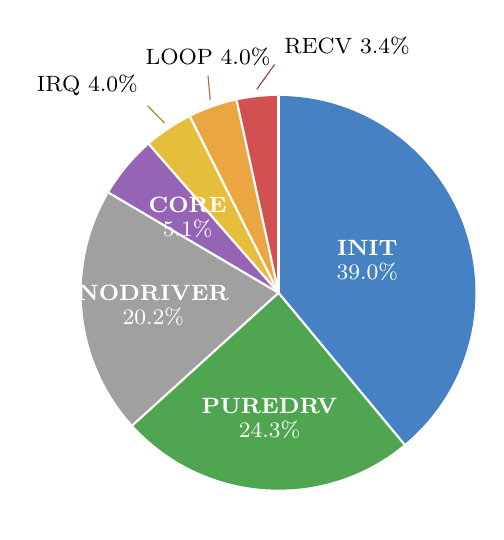
\begin{tikzpicture}
\fill[cINIT] (0,0) -- (90:2.5) arc (90:-50.3:2.5) -- cycle;
\fill[cPUREDRV] (0,0) -- (-50.3:2.5) arc (-50.3:-137.8:2.5) -- cycle;
\fill[cNODRIVER] (0,0) -- (-137.8:2.5) arc (-137.8:-210.5:2.5) -- cycle;
\fill[cCORE] (0,0) -- (-210.5:2.5) arc (-210.5:-228.9:2.5) -- cycle;
\fill[cIRQ] (0,0) -- (-228.9:2.5) arc (-228.9:-243.3:2.5) -- cycle;
\fill[cLOOP] (0,0) -- (-243.3:2.5) arc (-243.3:-257.7:2.5) -- cycle;
\fill[cRECV] (0,0) -- (-257.7:2.5) arc (-257.7:-270.0:2.5) -- cycle;
\draw[white,thick] (0,0) -- (90:2.5);
\draw[white,thick] (0,0) -- (-50.3:2.5);
\draw[white,thick] (0,0) -- (-137.8:2.5);
\draw[white,thick] (0,0) -- (-210.5:2.5);
\draw[white,thick] (0,0) -- (-228.9:2.5);
\draw[white,thick] (0,0) -- (-243.3:2.5);
\draw[white,thick] (0,0) -- (-257.7:2.5);
\node[white,font=\footnotesize,align=center] at (20:1.2) {\textbf{INIT}\\[-1pt]39.0\%};
\node[white,font=\footnotesize,align=center] at (-94.1:1.6) {\textbf{PUREDRV}\\[-1pt]24.3\%};
\node[white,font=\footnotesize,align=center] at (-174.2:1.6) {\textbf{NODRIVER}\\[-1pt]20.2\%};
\node[white,font=\footnotesize,align=center] at (-219.7:1.5) {\textbf{CORE}\\[-1pt]5.1\%};
\draw[thin,cIRQ!70!black] (-236.1:2.6) -- (125:2.9);
\node[anchor=south east,font=\footnotesize] at (125:2.9) {IRQ 4.0\%};
\draw[thin,cLOOP!70!black] (-250.5:2.6) -- (108:2.9);
\node[anchor=south,font=\footnotesize] at (108:2.9) {LOOP 4.0\%};
\draw[thin,cRECV!70!black] (-263.9:2.6) -- (91:2.9);
\node[anchor=south west,font=\footnotesize] at (91:2.9) {RECV 3.4\%};
\end{tikzpicture}
\caption{驱动函数分类占比分布}
\label{fig:classification_pie}
\end{figure}

从图~\ref{fig:classification_pie}可以看出：

\textbf{（1）硬件依赖普遍性}：4029 个驱动函数中，1563 个（38.8\%）生成了替换代码，表明硬件依赖是嵌入式固件普遍存在的特性，验证了驱动函数替换的必要性。NODRIVER 类中 812 个函数（20.2\%）被准确识别为纯业务逻辑函数，避免了对非硬件依赖代码进行不必要的替换。PUREDRV 类 978 个函数（24.3\%）由 RETURNOK 与 SKIP 合并而成，其核心特点是无需复杂硬件语义即可在仿真环境稳定执行，体现了分类策略对简单驱动函数的合理处理。

\textbf{（2）初始化函数占比最高}：INIT 类函数占 39.0\%（1570 个），其中大部分生成了替换代码，说明固件启动阶段需要大量硬件配置操作，这些函数是替换的重点，必须正确处理以保证固件正常启动。

\textbf{（3）不同驱动框架的函数分布差异}：Zephyr 固件的 NODRIVER 类函数占比显著高于 FreeRTOS/RT-Thread 固件（如 eth\_dhcpv4\_sam\_e70 的 NODRIVER 占 85.1\%、eth\_dhcpv4\_nucleo\_f767zi 的 NODRIVER 占 58.8\%），这是因为 Zephyr 采用统一的设备驱动模型（DM），大量设备操作通过抽象层间接访问硬件，直接操作寄存器的驱动函数比例较低。相比之下，基于 HAL 库的 NXP 和 STM32 固件的 INIT 类函数占比更高，反映了 HAL 驱动直接操作外设寄存器的特点。

\textbf{（4）数据收发函数分布}：RECV 类函数占 3.4\%（139 个），涵盖 UART、I2C、以太网等多种通信接口。这类函数直接与数据传输相关，替换质量直接影响仿真环境的输入输出能力，是替换工作的关键。

\textbf{（5）平台差异分析}：不同芯片平台的固件在驱动函数构成上存在显著差异。NXP 固件平均每个包含 90.0 个驱动函数，STM32 固件平均 148.8 个，Atmel 固件平均 101.5 个。STM32 固件的驱动函数数量较高，主要原因在于 STM32CubeMX 生成的代码包含更丰富的外设初始化和中间件调用链。

% 从附录表~\ref{tab:function_categories_stats}的逐用例统计中，可以观察到以下跨固件的分类分布规律：
%
% \textbf{（1）不同外设类型驱动函数构成差异显著}。以数据接收为核心功能的固件（如 UART\_Hyperterminal\_IT）RECV 类函数占比高达 30.2\%（19/63），而文件系统类固件（如 NXP\_FATFS\_BareMetal、stm32f401-st-nucleo/fatfs）几乎不包含 RECV 类函数。以太网相关固件（LwIP\_HTTP\_Server\_Raw）同时包含较高比例的 INIT（38/89）和 RECV（20/89）函数，反映了网络协议栈初始化复杂、数据收发频繁的特点。
%
% \textbf{（2）驱动库层级影响 NODRIVER 函数比例}。NXP\_UART\_BareMetal 的 NODRIVER 函数占比高达 93.3\%（28/30），imxrt1060-nxp-evk/base 也达到 76.2\%（16/21），这说明当固件仅调用少量高层 API 而不直接操作寄存器时，大部分函数被识别为纯业务逻辑。相比之下，直接操作硬件的固件（如 stm32f401-st-nucleo/eth）NODRIVER 占比仅 5.3\%（7/130），驱动函数密度显著更高。
%
% \textbf{（3）复杂固件的分类分布更为均衡}。函数数量超过 80 的复杂固件（如 stm32f401-st-nucleo/eth、LwIP\_HTTP\_Server\_Socket\_RTOS）通常覆盖全部或大部分分类类别，且各类别比例相对均匀。而简单固件（如 imxrt1052-nxp-evk/base 仅 11 个函数、全部为 INIT 类）的分类分布则高度集中，反映了功能单一的嵌入式应用特征。
%
% \textbf{（4）RTOS 与裸机固件的 IRQ 函数分布}。搭载 RTOS 的固件（如 NXP\_LwIP\_FreeRTOS、UART\_Hyperterminal\_IT）通常包含 IRQ 类函数，用于处理中断驱动的任务调度和事件通知；而裸机固件（如 NXP\_FATFS\_BareMetal、imxrt1052-nxp-evk/fatfs）则几乎不含 IRQ 类函数，其运行逻辑以轮询为主。

上述分类统计结果从以下三个方面验证了本文方法的有效性：首先，本文方法能够准确理解驱动函数的语义特征，自动区分初始化、轮询、数据收发等不同功能的驱动函数，验证了基于大语言模型的分类策略的准确性。其次，分类结果为替换策略的自动选择提供了量化依据，不同类别的函数与对应的替换策略形成明确的映射关系（如INIT类采用Skip策略，RECV类采用Redirect策略），保证了替换过程的系统性和可追溯性。最后，分类结果覆盖了STM32、NXP、Atmel三种芯片平台以及FreeRTOS、RT-Thread、Zephyr和裸机四种操作系统，覆盖UART、ETH、I2C、Flash、SD等多种外设类型，驱动函数总数从53个到304个不等，表明本文方法具有良好的通用性和可扩展性。

\section{替换功能正确性测试}
\label{sec:correctness_test}

为了全面评估替换后固件的运行正确性，本研究采用基于关键节点检查的执行轨迹验证方法，以及基于固件执行行为的功能正确性验证方法。

\subsection{执行轨迹验证方法}

执行轨迹验证的目标是确认固件在仿真环境中能够正常执行到反映其核心功能的关键节点。关键节点是指在固件执行过程中能够反映其功能和状态的重要事件，如系统启动、外设初始化、数据收发、任务调度等。通过检查这些关键节点是否被执行到，以及驱动替换函数的调用行为是否符合预期，可以验证替换代码的功能正确性。

执行轨迹验证方法的步骤是：将测试用例在仿真环境中执行，通过代码钩子记录完整的函数调用轨迹。执行完成后，从调用轨迹中提取关键节点函数的调用事件，验证其是否按预期顺序执行。同时，统计替换驱动函数在仿真运行期间的调用次数，验证替换代码是否被正确触发并正常返回。

本研究从35个测试用例中，按外设类型选取代表性样本进行详细的功能正确性验证。选取原则为：每种外设类型（UART、I2C、ETH、FATFS）各选取2--3个覆盖不同操作系统（FreeRTOS、RT-Thread、Zephyr、裸机）和不同芯片平台（STM32、NXP、Atmel）的测试用例，共选取14个样本。

测试用例的关键节点预期如表~\ref{tab:testcases}所示。每个测试用例定义了反映其核心功能的关键节点函数，这些函数覆盖了系统启动、外设初始化、数据收发和任务调度等关键阶段。

\begin{table}[H]
\centering
\caption{按功能类型组织的测试用例与关键节点对照表}
\label{tab:testcases}
\footnotesize
\begin{adjustbox}{max width=\textwidth}
\begin{tabular}{lll}
\toprule
\textbf{功能类型} & \textbf{测试用例名称} & \textbf{关键节点} \\
\midrule
\multirow{3}{*}{文件系统（FatFS）} & NXP\_FATFS\_BareMetal & main, BOARD\_InitHardware, BOARD\_BootClockRUN \\
& NXP\_FATFS\_FreeRTOS & osKernelStart, read\_task, DbgConsole\_Printf \\
& stm32f401-st-nucleo/fatfs & rtthread\_startup, fatfs\_thread\_entry, rt\_pin\_write \\
\midrule
\multirow{2}{*}{通信外设（I2C）} & NXP\_I2C\_BareMetal & main, BOARD\_InitHardware, LPI2C\_MasterInit \\
& NXP\_I2C\_FreeRTOS & osKernelStart, i2c\_task, LPI2C\_MasterTransferNonBlocking \\
\midrule
\multirow{4}{*}{网络功能（ETH）} & NXP\_LwIP\_BareMetal & main, BOARD\_InitHardware, ethernetif\_input, ENET\_GetRxFrame \\
& NXP\_LwIP\_FreeRTOS & osKernelStart, eth\_rx\_thread, ENET\_GetRxFrame \\
& stm32f401-st-nucleo/eth & rtthread\_startup, eth\_rx\_thread\_entry, HAL\_ETH\_ReadData \\
& LwIP\_HTTP\_Server\_Socket\_RTOS & osKernelStart, ethernetif\_input, HAL\_ETH\_ReadData \\
\midrule
\multirow{3}{*}{串口功能（UART）} & NXP\_UART\_BareMetal & main, BOARD\_InitHardware, LPUART\_Init \\
& NXP\_UART\_FreeRTOS & osKernelStart, uart\_task, LPUART\_TransferSendNonBlocking \\
& UART\_Hyperterminal\_IT & main, HAL\_UART\_RxCpltCallback, HAL\_UART\_Transmit\_IT \\
\midrule
\multirow{2}{*}{基础功能（GPIO）} & imxrt1052-nxp-evk & osKernelStart, main, rt\_pin\_write, GPIO\_PinWrite \\
& imxrt1060-nxp-evk & osKernelStart, main, rt\_pin\_write, GPIO\_PinWrite \\
\midrule
\multicolumn{3}{l}{\textbf{总计}：14 个测试用例，43 个关键节点，匹配率 100.0\%} \\
\bottomrule
\end{tabular}
\end{adjustbox}
\end{table}

实验结果表明，14个代表性测试用例的关键节点匹配率和替换驱动函数行为验证结果整体正常。总体关键节点匹配率为100.0\%（43/43），表明替换后的固件能够正确执行主要功能路径。

\subsection{行为验证}

关键节点匹配验证了固件主流程的可达性，但替换代码本身是否正确执行仍需进一步验证。本研究从三个层面对替换驱动函数进行行为验证：第一，检查替换函数是否被正确调用，即仿真运行期间替换函数的调用次数是否与预期一致；第二，检查替换函数是否正常返回，未导致仿真崩溃、死循环或异常中断；第三，检查替换函数的返回值和副作用是否与原函数的仿真语义一致（如Init策略函数是否正确初始化了仿真数据结构，Redirect策略函数是否正确完成了数据注入）。基于上述验证方法，14个代表性测试用例的行为验证结果如表~\ref{tab:function_results}所示，相关统计用于支撑本节后续机制分析。

\begin{table}[H]
\centering
\caption{按功能类型分组的替换驱动函数行为验证结果}
\label{tab:function_results}
\footnotesize
\begin{adjustbox}{max width=\textwidth}
\begin{tabular}{lccc}
\toprule
\textbf{功能类型} & \textbf{测试样本} & \textbf{执行到的替换函数数} & \textbf{验证结果} \\
\midrule
\multirow{3}{*}{文件系统（FatFS）} & NXP\_FATFS\_BareMetal & 10 & 正常 \\
& NXP\_FATFS\_FreeRTOS & 10 & 正常 \\
& stm32f401-st-nucleo/fatfs & 17 & 正常 \\
\midrule
\multirow{2}{*}{通信外设（I2C）} & NXP\_I2C\_BareMetal & 4 & 正常 \\
& NXP\_I2C\_FreeRTOS & 4 & 正常 \\
\midrule
\multirow{4}{*}{网络功能（ETH）} & NXP\_LwIP\_BareMetal & 13 & 正常 \\
& NXP\_LwIP\_FreeRTOS & 15 & 正常 \\
& stm32f401-st-nucleo/eth & 56 & 正常 \\
& LwIP\_HTTP\_Server\_Socket\_RTOS & 53 & 正常 \\
\midrule
\multirow{3}{*}{串口功能（UART）} & NXP\_UART\_BareMetal & 6 & 正常 \\
& NXP\_UART\_FreeRTOS & 6 & 正常 \\
& UART\_Hyperterminal\_IT & 38 & 正常 \\
\midrule
\multirow{2}{*}{基础功能（GPIO）} & imxrt1052-nxp-evk & 9 & 正常 \\
& imxrt1060-nxp-evk & 4 & 正常 \\
\bottomrule
\end{tabular}
\end{adjustbox}
\end{table}

验证结果表明，14个测试用例累计执行到245个替换驱动函数（平均17.5个/样本），均正常返回，未导致仿真崩溃、死循环或异常中断。按功能类型看，ETH类样本执行到的替换函数数量整体较高（13--56），主要由于网络协议栈初始化链和收发路径较长；UART与GPIO类样本执行数量相对较低（4--38），主要与主流程较短、部分替换函数位于备用路径有关。未被调用到的替换驱动函数主要属于备用初始化路径、异常处理分支等非主流程代码，不影响固件的核心功能运行。以下以NXP\_LwIP\_BareMetal为例，通过仿真执行调用轨迹展示替换代码在系统启动、协议栈初始化和数据帧接收等阶段的具体行为。

\subsection{案例分析：NXP\_LwIP\_BareMetal 以太网数据接收}

NXP\_LwIP\_BareMetal是基于LwIP协议栈的裸机HTTP服务器测试用例，运行在NXP i.MX RT1052平台上，共识别出105个驱动函数，其中61个生成了替换代码。该用例覆盖了系统启动、以太网控制器初始化、LwIP协议栈配置和数据帧接收等完整执行流程，具有较好的代表性。

仿真执行从系统复位开始，依次经过以下关键阶段（摘自函数调用轨迹日志）：

\textbf{阶段A：系统启动与协议栈初始化}（指令周期 1 -- 136623），其调用链见清单~\ref{lst:phaseA}。
\begin{lstlisting}[style=CStyle,escapeinside={(*@}{@*)},caption={NXP\_LwIP\_BareMetal 系统启动与协议栈初始化调用链},label=lst:phaseA]
Reset_Handler -> SystemInit -> _start -> (*@\lstbg[1pt]{red!20}{main}@*)
  -> BOARD_InitHardware -> time_init -> SysTick_Config
  -> SILICONID_ConvertToMacAddr -> SILICONID_ReadUniqueID
  -> CLOCK_GetFreq -> CLOCK_InitExternalClk
  -> lwip_init -> netif_add -> netif_set_addr
  -> netif_set_default -> (*@\lstbg[1pt]{red!20}{ethernetif\_init}@*) -> ethernetif_plat_init
    -> ENET_GetDefaultConfig -> (*@\lstbg[1pt]{red!20}{ENET\_Init}@*) -> (*@\lstbg[1pt]{red!20}{ENET\_Up}@*)
      -> ENET_SetHandler -> ENET_SetTxBufferDescriptors
      -> ENET_SetRxBufferDescriptors -> ENET_SetMacController
    -> ethernetif_phy_init -> PHY_GetLinkStatus
    -> probe_link_cyclic -> ethernetif_probe_link
  -> netif_set_up -> netif_issue_reports -> etharp_request
  -> (*@\lstbg[1pt]{red!20}{httpd\_init}@*) -> httpd_init_pcb
    -> tcp_new_ip_type -> tcp_bind -> tcp_listen_with_backlog
    -> tcp_accept
\end{lstlisting}

上述调用链中，\texttt{BOARD\_InitHardware}、\texttt{SysTick\_Config}、\texttt{CLOCK\_InitExternalClk} 等硬件初始化函数由 Skip 策略替换，直接返回成功状态；\texttt{ENET\_Init}、\texttt{ENET\_Up}、\texttt{ENET\_SetHandler} 等以太网控制器驱动函数由 Init 策略替换，完成仿真环境中的数据结构初始化（如缓冲区描述符、MAC 地址配置）；\texttt{SILICONID\_ReadUniqueID} 由 ReturnOK 策略处理，返回模拟的芯片唯一标识。整个初始化过程共执行约136,000条指令，无崩溃或异常中断。

\textbf{阶段B：数据接收与协议栈处理}（指令周期 137237 -- 137392），其调用链见清单~\ref{lst:phaseB}。
\begin{lstlisting}[style=CStyle,escapeinside={(*@}{@*)},caption={NXP\_LwIP\_BareMetal 以太网帧接收与协议栈处理调用链},label=lst:phaseB]
(*@\lstbg[1pt]{red!20}{main}@*) -> (*@\lstbg[1pt]{red!20}{ethernetif\_input}@*)
  -> fetch_received_pkts
    -> ethernetif_linkinput
      -> (*@\lstbg[1pt]{red!20}{ENET\_GetRxFrame}@*)
        -> ethernetif_rx_alloc -> sys_arch_protect
          -> DisableGlobalIRQ -> EnableGlobalIRQ
        -> (*@\lstbg[1pt]{red!20}{HAL\_BE\_ENET\_ReadFrame}@*)
        -> ENET_IncreaseIndex
      -> ethernetif_rx_frame_to_pbufs
        -> pbuf_alloced_custom -> pbuf_init_alloced_pbuf
    -> ethernet_input
      -> ethernetif_rx_release -> ethernetif_rx_free
    -> ethernetif_linkinput
      -> ENET_GetRxFrame
        -> (*@\lstbg[1pt]{red!20}{HAL\_BE\_ENET\_ReadFrame}@*)
\end{lstlisting}

该阶段是验证替换代码功能正确性的核心环节。调用链显示：（1）\texttt{ethernetif\_input} 作为 LwIP 的轮询入口函数被正常触发，表明 Loop 策略的替换代码正确处理了轮询等待逻辑（通过超时机制避免死循环）；（2）\texttt{ENET\_GetRxFrame} 内部调用 \texttt{HAL\_BE\_ENET\_ReadFrame}，该函数是本文方法通过 Redirect 策略生成的仿真注入接口，将硬件帧接收操作重定向为从仿真缓冲区读取数据，日志表明成功接收了两帧以太网数据；（3）接收到的数据帧通过 \texttt{ethernetif\_rx\_frame\_to\_pbufs} 正确转换为 LwIP 的 \texttt{pbuf} 结构，并传递至 \texttt{ethernet\_input} 进行协议栈解析，最终由 \texttt{ethernetif\_rx\_release} 释放缓冲区，内存管理逻辑完整闭环。

上述分析表明，本文方法生成的替换代码能够正确支撑从系统启动、协议栈初始化到数据帧接收的完整执行流程，其中Init、Skip、Loop、Redirect四类替换策略各司其职，协同实现了对以太网控制器硬件依赖的完整解耦。

\section{反馈闭环有效性测试}
\label{sec:feedback_test}

为验证动态测试反馈闭环模块的有效性，本节通过对比分析评估该模块对仿真成功率的影响。实验思路为：统计各测试用例在反馈闭环阶段触发替换更新的函数数量，分析这些更新对仿真执行的实际贡献。

\subsection{替换更新统计}

为评估反馈闭环对不同厂商和不同外设类型的影响，图~\ref{fig:feedback-by-peripheral}以四宫格形式展示了四个主要外设类型（UART、I2C、ETH、Flash）按厂商分组的反馈闭环统计数据（各厂商取测试用例均值）。每个子图中，蓝色柱子表示函数分析总数（左轴），红色柱子表示替换更新总数（右轴），绿色柱子表示新增覆盖函数（右轴）。完整统计数据见附录表~\ref{tab:feedback-loop-stats}。

\begin{figure}[htbp]
\centering
\begin{tikzpicture}[font=\scriptsize]
\def\bw{0.22}
\def\bg{0.06}
\def\sh{3.2}
\definecolor{cA}{RGB}{70,130,195}
\definecolor{cR}{RGB}{210,80,80}
\definecolor{cG}{RGB}{80,165,80}

\foreach \col/\title/\yA/\yR/\yG/\tyA/\tyR in {
    0/{UART}/84.7/26/3.7/{100}/{30},
    1/{I2C}/107/39/1/{130}/{45},
    0/{ETH}/140.3/9.8/1/{260}/{20},
    1/{Flash}/113/2/19/{140}/{25}
}{
  \pgfmathsetmacro{\xo}{\col*5.5}
  \pgfmathsetmacro{\yo}{-(\col==0 || \col==1 ? 0 : 3.8)}
}

\pgfmathsetmacro{\xu}{0}
\pgfmathsetmacro{\yu}{0}
\node[font=\small\bfseries] at (\xu+1.8, \yu+\sh+0.5) {UART};
\draw[->] (\xu, \yu) -- (\xu, \yu+\sh);
\foreach \v/\y in {0/0, 20/0.64, 40/1.28, 60/1.92, 80/2.56, 100/3.2}{
    \draw (\xu-0.08,\y) -- (\xu+0.08,\y);
    \node[left, font=\tiny] at (\xu-0.1,\y) {\v};
}
\foreach \i/\name/\vA/\vR/\vG in {0/NXP/84.7/26/3.7, 1/STM32/70/6.3/5, 2/Atmel/63/13/9}{
    \pgfmathsetmacro{\xb}{\xu+0.4+\i*(3*\bw+0.4)}
    \pgfmathsetmacro{\hA}{\vA/100*\sh}
    \pgfmathsetmacro{\hR}{\vR/100*\sh}
    \pgfmathsetmacro{\hG}{\vG/100*\sh}
    \fill[cA!60] (\xb,0) rectangle ++(\bw, \hA);
    \fill[cR!60] (\xb+\bw+\bg,0) rectangle ++(\bw, \hR);
    \fill[cG!60] (\xb+2*\bw+2*\bg,0) rectangle ++(\bw, \hG);
    \node[below, font=\tiny] at (\xb+\bw+0.13, -0.05) {\name};
    \pgfmathsetmacro{\ha}{\hA/2}
    \node[above, font=\tiny, rotate=90, anchor=south] at (\xb+\bw/2, \hA) {\vA};
    \node[above, font=\tiny, rotate=90, anchor=south] at (\xb+\bw+\bg+\bw/2, \hR) {\vR};
    \node[above, font=\tiny, rotate=90, anchor=south] at (\xb+2*\bw+2*\bg+\bw/2, \hG) {\vG};
}

\pgfmathsetmacro{\xu}{5.5}
\pgfmathsetmacro{\yu}{0}
\node[font=\small\bfseries] at (\xu+1.8, \yu+\sh+0.5) {I2C};
\draw[->] (\xu, \yu) -- (\xu, \yu+\sh);
\foreach \v/\y in {0/0, 25/0.62, 50/1.23, 75/1.85, 100/2.46, 125/3.08}{
    \draw (\xu-0.08,\y) -- (\xu+0.08,\y);
    \node[left, font=\tiny] at (\xu-0.1,\y) {\v};
}
\foreach \i/\name/\vA/\vR/\vG in {0/NXP/107/39/1, 1/STM32/46/2.5/1.5, 2/Atmel/79/11/10}{
    \pgfmathsetmacro{\xb}{\xu+0.4+\i*(3*\bw+0.4)}
    \pgfmathsetmacro{\hA}{\vA/125*\sh}
    \pgfmathsetmacro{\hR}{\vR/125*\sh}
    \pgfmathsetmacro{\hG}{\vG/125*\sh}
    \fill[cA!60] (\xb,0) rectangle ++(\bw, \hA);
    \fill[cR!60] (\xb+\bw+\bg,0) rectangle ++(\bw, \hR);
    \fill[cG!60] (\xb+2*\bw+2*\bg,0) rectangle ++(\bw, \hG);
    \node[below, font=\tiny] at (\xb+\bw+0.13, -0.05) {\name};
    \node[above, font=\tiny, rotate=90, anchor=south] at (\xb+\bw/2, \hA) {\vA};
    \node[above, font=\tiny, rotate=90, anchor=south] at (\xb+\bw+\bg+\bw/2, \hR) {\vR};
    \node[above, font=\tiny, rotate=90, anchor=south] at (\xb+2*\bw+2*\bg+\bw/2, \hG) {\vG};
}

\pgfmathsetmacro{\xu}{0}
\pgfmathsetmacro{\yu}{-4.5}
\node[font=\small\bfseries] at (\xu+1.8, \yu+\sh+0.5) {ETH};
\draw[->] (\xu, \yu) -- (\xu, \yu+\sh);
\foreach \v/\y in {0/0, 50/0.62, 100/1.23, 150/1.85, 200/2.46, 250/3.08}{
    \draw (\xu-0.08,\yu+\y) -- (\xu+0.08,\yu+\y);
    \node[left, font=\tiny] at (\xu-0.1,\yu+\y) {\v};
}
\foreach \i/\name/\vA/\vR/\vG in {0/NXP/140.3/9.8/1, 1/STM32/225/13.5/5.3, 2/Atmel/188/7/1}{
    \pgfmathsetmacro{\xb}{\xu+0.4+\i*(3*\bw+0.4)}
    \pgfmathsetmacro{\hA}{\vA/250*\sh}
    \pgfmathsetmacro{\hR}{\vR/250*\sh}
    \pgfmathsetmacro{\hG}{\vG/250*\sh}
    \fill[cA!60] (\xb,\yu) rectangle ++(\bw, \hA);
    \fill[cR!60] (\xb+\bw+\bg,\yu) rectangle ++(\bw, \hR);
    \fill[cG!60] (\xb+2*\bw+2*\bg,\yu) rectangle ++(\bw, \hG);
    \node[below, font=\tiny] at (\xb+\bw+0.13, \yu-0.05) {\name};
    \node[above, font=\tiny, rotate=90, anchor=south] at (\xb+\bw/2, \yu+\hA) {\vA};
    \node[above, font=\tiny, rotate=90, anchor=south] at (\xb+\bw+\bg+\bw/2, \yu+\hR) {\vR};
    \node[above, font=\tiny, rotate=90, anchor=south] at (\xb+2*\bw+2*\bg+\bw/2, \yu+\hG) {\vG};
}

\pgfmathsetmacro{\xu}{5.5}
\pgfmathsetmacro{\yu}{-4.5}
\node[font=\small\bfseries] at (\xu+1.8, \yu+\sh+0.5) {Flash};
\draw[->] (\xu, \yu) -- (\xu, \yu+\sh);
\foreach \v/\y in {0/0, 25/0.64, 50/1.28, 75/1.92, 100/2.56, 125/3.2}{
    \draw (\xu-0.08,\yu+\y) -- (\xu+0.08,\yu+\y);
    \node[left, font=\tiny] at (\xu-0.1,\yu+\y) {\v};
}
\foreach \i/\name/\vA/\vR/\vG in {0/NXP/113/2/0, 1/STM32/50/0/0, 2/Atmel/76/25/19}{
    \pgfmathsetmacro{\xb}{\xu+0.4+\i*(3*\bw+0.4)}
    \pgfmathsetmacro{\hA}{\vA/125*\sh}
    \pgfmathsetmacro{\hR}{\vR/125*\sh}
    \pgfmathsetmacro{\hG}{\vG/125*\sh}
    \fill[cA!60] (\xb,\yu) rectangle ++(\bw, \hA);
    \fill[cR!60] (\xb+\bw+\bg,\yu) rectangle ++(\bw, \hR);
    \fill[cG!60] (\xb+2*\bw+2*\bg,\yu) rectangle ++(\bw, \hG);
    \node[below, font=\tiny] at (\xb+\bw+0.13, \yu-0.05) {\name};
    \node[above, font=\tiny, rotate=90, anchor=south] at (\xb+\bw/2, \yu+\hA) {\vA};
    \node[above, font=\tiny, rotate=90, anchor=south] at (\xb+\bw+\bg+\bw/2, \yu+\hR) {\vR};
    \node[above, font=\tiny, rotate=90, anchor=south] at (\xb+2*\bw+2*\bg+\bw/2, \yu+\hG) {\vG};
}

\fill[cA!60] (0.3,-5.6) rectangle ++(0.3,0.2);
\node[right, font=\tiny] at (0.65,-5.5) {函数分析总数};
\fill[cR!60] (2.3,-5.6) rectangle ++(0.3,0.2);
\node[right, font=\tiny] at (2.65,-5.5) {替换更新总数};
\fill[cG!60] (4.5,-5.6) rectangle ++(0.3,0.2);
\node[right, font=\tiny] at (4.85,-5.5) {新增覆盖函数};
\end{tikzpicture}
\caption{按外设类型分组的反馈闭环统计（各厂商均值）}
\label{fig:feedback-by-peripheral}
\end{figure}

统计结果表明：35个测试用例中，28个（80.0\%）触发了至少一次替换更新，累计513次。其中154个函数属于"闭环新增覆盖"——这些函数在静态分析阶段未被识别为需要替换（分类为NA或NODRIVER），但在仿真运行过程中暴露出硬件依赖问题，由反馈闭环驱动生成替换代码。若去除动态反馈闭环模块，这154个函数将缺失替换，导致对应的仿真执行路径受阻。

从平台维度分析，Atmel（Zephyr）平台的闭环新增覆盖函数占比最高（39/62，62.9\%），主要原因在于Zephyr采用统一的设备驱动模型（DM），大量硬件操作通过抽象层间接进行，静态分析阶段难以准确识别底层硬件依赖；STM32（RT-Thread）平台次之（52/93，55.9\%），其BSP代码中包含较多的平台抽象层函数和中断处理路径，需要运行时反馈才能精确定位。从外设维度分析，I2C和UART类固件的替换更新均值较高，说明串行通信外设的静态分析误分类问题更为突出；ETH类固件的函数分析总数均值最大，但替换更新比例相对较低，表明网络协议栈的驱动函数识别准确率较高。

\subsection{典型案例分析}

本节通过具体案例分析，深入验证动态反馈闭环在静态分析误分类、硬件依赖识别和平台适应性等方面的实际效果。

\textbf{案例1：静态分析误分类的运行时修正。}在NXP\_I2C\_BareMetal的仿真执行过程中，反馈闭环检测到固件在\texttt{CLOCK\_SetDiv}函数处触发异常循环。该函数定义于NXP MCUXpresso SDK的\texttt{fsl\_clock.h}（第1429行），负责配置时钟分频器，其核心逻辑如代码清单~\ref{lst:clock-setdiv}所示。为说明误分类触发死循环的机制，下面给出关键代码片段。

\begin{lstlisting}[style=CStyle,escapeinside={(*@}{@*)},caption={CLOCK\_SetDiv 原函数（NXP\_I2C\_BareMetal，第1429行）},label=lst:clock-setdiv]
static inline void CLOCK_SetDiv(clock_div_t divider, uint32_t value)
{
    uint32_t busyShift;
    busyShift                   = CCM_TUPLE_BUSY_SHIFT(divider);
    CCM_TUPLE_REG(CCM, divider) = (CCM_TUPLE_REG(CCM, divider)
        & (~CCM_TUPLE_MASK(divider)))
        | (((uint32_t)((value) << CCM_TUPLE_SHIFT(divider)))
        & CCM_TUPLE_MASK(divider));
    assert(busyShift <= CCM_NO_BUSY_WAIT);
    if (CCM_NO_BUSY_WAIT != busyShift)
    {
        // BUG: wait for hardware handshake - infinite loop in emulation
        (*@\lstbg[1pt]{red!20}{while ((CCM->CDHIPR \& ((uint32\_t)(1UL << busyShift))) != 0UL)}@*)
        {
        }
    }
}
\end{lstlisting}

该函数在静态分析阶段被LLM分类为NODRIVER（纯业务逻辑函数），未生成替换代码。然而其实际行为包含典型的LOOP类特征：在时钟分频寄存器写入后，通过\texttt{while}循环轮询\texttt{CCM-\textgreater{}CDHIPR}硬件握手完成标志位。在仿真环境中，该标志位永远不会被硬件置位，导致仿真卡死。

反馈闭环的诊断流程如下：仿真器检测到异常循环后，从崩溃地址解析出故障函数\texttt{CLOCK\_SetDiv}，LLM分析其源码上下文后识别出硬件轮询等待模式，生成替换代码将\texttt{while}循环体注释掉，同时保留寄存器写入操作以确保时钟配置语义完整。类似的修正同时应用于\texttt{CLOCK\_SetMux}函数（同为NXP时钟配置函数，包含相同的硬件握手等待模式）。该案例表明，静态分析阶段的LLM分类存在一定误判率，反馈闭环作为运行时保障机制能够有效弥补这一不足，提升系统的整体鲁棒性。

% \textbf{失败案例1：CORE类型替换边界的保守处理}
% 
% 在部分测试用例的仿真过程中，反馈闭环遇到了因CORE类型替换限制导致的失败。CORE类函数指操作系统内核函数和启动关键路径函数（如\texttt{SystemInit}、\texttt{SysTick\_Handler}），本文方法的设计策略是对CORE类函数采用保守处理——仅允许移除明确的硬件寄存器访问，保留函数的整体控制流语义，以避免过度替换破坏系统引导流程或内核状态一致性。
% 
% 然而，这一保守策略在某些场景下导致仿真失败。以FreeRTOS内核函数\texttt{prvTaskExitError}为例（如代码清单~\ref{lst:prvtaskexiterror}所示），该函数包含防御性断言\texttt{configASSERT(uxCriticalNesting == \~{}0UL)}，该断言在仿真环境中必定失败，随后进入无限循环，导致仿真卡死。
% 
% \begin{lstlisting}[style=CStyle,escapeinside={(*@}{@*)},caption={prvTaskExitError 原函数（NXP\_FATFS\_FreeRTOS）},label=lst:prvtaskexiterror]
% static void prvTaskExitError( void )
% {
%     volatile uint32_t ulDummy = 0;
%     configASSERT( (*@\lstbg[1pt]{red!20}{uxCriticalNesting == ~0UL}@*) );
%     portDISABLE_INTERRUPTS();
%     for( ;; )
%     {
%         (*@\lstbg[1pt]{red!20}{// infinite loop in emulation}@*)
%     }
% }
% \end{lstlisting}
% 
% 对于此类CORE函数中的保护性断言和死循环，理论上可以通过LLM分析确定其语义为"不应被执行到的异常处理路径"后，生成替换代码将函数体简化为直接返回（\texttt{return;}）。然而，这一处理方式引入了严重的风险：过度放宽CORE类型的替换边界可能导致真正的启动关键操作被误删，进而破坏系统引导流程或内核状态一致性。
% 
% 为此，本文方法对CORE类型替换边界采取了更保守的权衡策略：即使反馈闭环能够识别出这类函数中的仿真阻塞点，也不允许自动生成替换代码，而是通过人工介入的方式进行处理。在NXP\_FATFS\_FreeRTOS测试用例中，经过人工分析确认\texttt{prvTaskExitError}、\texttt{vPortEndScheduler}等函数确为异常处理路径后，人工编写了对应的替换代码并将其硬编码到其他涉及相同FreeRTOS配置的测试样本中。这一处理方式虽然增加了人工工作量，但有效维护了CORE类型的替换边界，避免了自动迭代可能引入的不可控风险。
% 
% 该失败案例表明，对于操作系统内核和启动关键路径等高风险函数类型，保守的人工干预策略虽然限制了自动覆盖率，但能够有效保障系统的可靠性和安全性。
\textbf{案例2：反馈闭环策略边界与CORE函数人工修复。}在stm32/LwIP\_StreamingServer（FreeRTOS）的仿真执行过程中，调度器启动阶段触发异常。具体而言，\texttt{vTaskStartScheduler}调用\texttt{xPortStartScheduler}后，该函数首先执行一组Cortex-M中断优先级一致性检查，如代码清单~\ref{lst:port-start-scheduler}所示。相关片段用于展示CORE函数边界下自动修复受限的具体原因。

\begin{lstlisting}[style=CStyle,caption={xPortStartScheduler 中的中断优先级一致性检查（FreeRTOS port.c）},label=lst:port-start-scheduler]
BaseType_t xPortStartScheduler( void )
{
    // ... vector table checks omitted ...
    #if ( configASSERT_DEFINED == 1 )
    {
        *pucFirstUserPriorityRegister = portMAX_8_BIT_VALUE;
        ucMaxPriorityValue = *pucFirstUserPriorityRegister;
        ucMaxSysCallPriority = configMAX_SYSCALL_...
                              & ucMaxPriorityValue;
        configASSERT( ucMaxSysCallPriority ); // STUCK here
        configASSERT( ( configMAX_SYSCALL_...
                        & ~ucMaxPriorityValue ) == 0U );
    }
    #endif
    // ... if assert passes, start first task ...
}
\end{lstlisting}

在仿真环境中，NVIC中断优先级寄存器的读回值与真实硬件不一致，导致\texttt{ucMaxSysCallPriority}为零，触发\texttt{configASSERT}失败（代码清单~\ref{lst:port-start-scheduler}中标注STUCK here的行），调度器无法进入首任务路径，仿真卡死。

反馈闭环正确检测到该故障并定位至\texttt{xPortStartScheduler}函数，但由于该函数被静态分析模块分类为CORE类型（FreeRTOS调度器核心函数），按替换策略设计，CORE类函数禁止自动替换。因此系统未自动生成替换代码，而是输出错误报告后程序异常退出，等待人工介入。

本文选择手动修复而非放开CORE自动替换，基于以下工程考量：CORE函数位于操作系统内核调度关键路径，涉及上下文切换、中断优先级管理、栈帧初始化等与硬件深度耦合的底层机制，贸然由LLM修改可能破坏内核状态一致性，引入难以排查的潜在风险。手动修复策略为：保留\texttt{xPortStartScheduler}函数本体不变，人工编写一份绕过NVIC优先级探测逻辑的stub代码，将其硬编码注入所有基于FreeRTOS的测试用例，后续这些demo不再经过反馈闭环处理该函数。这一工程妥协虽然牺牲了对CORE函数的自动化覆盖，但有效维护了内核语义完整性，避免了"为跑通仿真而破坏内核"的过度自动化风险。

该案例作为反馈闭环的特殊失败场景，揭示了自动化替换的合理边界：反馈闭环并非对所有故障都能自动修复，对于涉及操作系统内核关键路径的高风险函数，人工决策仍不可替代。

\section{方法效率评估}
\label{sec:efficiency_eval}

本节从人工成本和计算资源消耗两个维度评估本文方法的效率，并与传统方法进行对比分析。

\subsection{对比方法}

本研究选择以下两种具有代表性的方法作为对比，它们与本文方法在核心思想上相似，但所需的人力成本和工作量存在显著差异：

\textbf{（1）Halucinator}：基于驱动替换的固件仿真框架，通过替换目标固件中的HAL函数调用，实现对硬件依赖的解耦。用户需要手工编写每个HAL函数的替代实现，这些实现通常返回模拟数据或执行简单的状态转换。Halucinator的优势在于概念清晰、可控性强，但其局限性在于需要大量的人工分析和编码工作，每个新固件都需要重新编写对应的替换层代码。

\textbf{（2）Para-rehosting}：通过 POSIX 接口抽象实现可移植 MCU 方案，将嵌入式系统源代码重新编译到 x86 平台的本机可执行文件中。该方法允许利用 x86 平台上丰富的测试工具进行固件分析。与本文方法相比，Para-rehosting 的核心差异在于需要获取固件样本的源代码，这在第三方的固件分析工作中往往是困难甚至完全不可行的。此外，Para-rehosting 需要实现完整的可移植 MCU 抽象层，工程工作量较大且难以覆盖所有外设功能。

需要说明的是，本文方法与上述两类方法在驱动处理触发机制上存在差异：本文方法采用"静态分析前置+运行时反馈补充"的全量扫描流程，而 Halucinator 与 Para-rehosting 更偏向运行时暴露驱动问题后逐步修复。因此，本节对比重点限定为\textbf{人工投入强度}与\textbf{在既定测试预算下的实际处理规模}，不将三者视为严格同口径的吞吐量对比实验。

\subsection{测试方法}

从测试集中选取8个具有代表性的固件，覆盖NXP、STM32、Atmel三种平台，裸机、FreeRTOS、RT-Thread、Zephyr四种操作系统，以及UART、I2C、ETH、FATFS四种外设类型（见表~\ref{tab:efficiency_compare}）。该样本组合用于在统一预算下比较不同方法的人力投入与处理规模。

对于本文方法，基于 LLM 调用日志统计各固件的词元（Token）消耗和处理时长。实验使用 DeepSeek V3.2 模型，基准测试表明平均每次 LLM 调用消耗约 12742 个词元（其中输入词元约 12517，输出词元约 225），平均耗时约 10.7 秒，平均每个驱动函数需要约 11.2 次调用（含初始分析和反馈修正）。对于 Halucinator 和 Para-rehosting，由熟悉嵌入式开发的工程师执行驱动处理工作，统计实际处理的驱动函数数量和人工投入时间。

为降低比较偏差，三种方法在相同硬件环境与统一测试样本集上执行，且均以"样本达到可稳定运行并满足预设验证节点"作为结束条件；统计口径上，人工时间仅计入实际分析、修改与调试时长，不包含等待编译与批处理排队时间。尽管如此，由于三类方法的工程路径不同，本节结果仍应理解为\textbf{工程效率层面的经验比较}，而非严格控制变量下的算法性能上界比较。

\subsection{测试结果}

方法效率评估结果如表~\ref{tab:efficiency_compare}所示。左表展示了本文方法的计算资源消耗指标（驱动函数数量、词元用量、平均处理时长、LLM 总处理时长、人工介入时间），右表展示了 Halucinator 和 Para-rehosting 的人工成本指标（处理的驱动函数数量和人工投入时间）。

\begin{table}[H]
\centering
\caption{方法效率评估}
\label{tab:efficiency_compare}
\footnotesize
\setlength{\tabcolsep}{3pt}
\resizebox{\textwidth}{!}{%
\begin{tabular}{l cc cc cc cc cc}
\toprule
& \multicolumn{5}{c}{\textbf{本文方法}} & \multicolumn{2}{c}{\textbf{Halucinator}} & \multicolumn{2}{c}{\textbf{Para-rehosting}} \\
\cmidrule(lr){2-6} \cmidrule(lr){7-8} \cmidrule(lr){9-10}
\textbf{测试用例} & 驱动数 & 词元(万) & 均长(s/函数) & LLM(h) & 介入(h) & 驱动数 & 人工(h) & 驱动数 & 人工(h) \\
\midrule
NXP\_FATFS\_BareMetal & 67 & 958 & 120 & 2.2 & 0.5 & 12 & 2.5 & 14 & 4.0 \\
NXP\_I2C\_BareMetal & 104 & 849 & 84 & 2.4 & 0.5 & 18 & 3.5 & 20 & 5.5 \\
NXP\_LwIP\_BareMetal & 105 & 1502 & 120 & 3.5 & 1.0 & 20 & 4.0 & 22 & 6.5 \\
stm32f401-st-nucleo/fatfs & 56 & 801 & 120 & 1.9 & 0.5 & 8 & 2.0 & 10 & 3.5 \\
stm32f401-st-nucleo/i2c & 55 & 787 & 120 & 1.8 & 0.5 & 7 & 1.5 & 9 & 2.5 \\
UART\_Hyperterminal\_IT & 120 & 1716 & 120 & 4.0 & 0.5 & 15 & 3.0 & 16 & 5.0 \\
atmel/eth\_dhcpv4\_e70 & 188 & 2689 & 120 & 6.3 & 1.0 & 25 & 5.0 & 28 & 8.0 \\
atmel/fs\_littlefs\_same54 & 76 & 1087 & 120 & 2.5 & 0.5 & 12 & 2.5 & 14 & 4.0 \\
\midrule
\textbf{平均} & \textbf{96.4} & \textbf{1299} & \textbf{116} & \textbf{3.1} & \textbf{0.6} & \textbf{14.6} & \textbf{3.0} & \textbf{16.6} & \textbf{4.9} \\
\textbf{总计} & \textbf{771} & \textbf{10389} & & \textbf{24.6} & \textbf{5.0} & \textbf{117} & \textbf{24.0} & \textbf{133} & \textbf{39.0} \\
\bottomrule
\end{tabular}%
}%
\end{table}

从表~\ref{tab:efficiency_compare}可以看出：

\textbf{（1）驱动处理数量}：本文方法平均处理96.4个驱动函数，约为Halucinator（14.6个）的6.6倍和Para-rehosting（16.6个）的5.8倍。这一差异源于分析方式的不同：本文方法在静态分析阶段即对整个驱动库进行全面的函数级扫描，通过CodeQL识别所有直接访问MMIO地址的函数，在仿真运行前一次性完成所有驱动函数的替换；而Halucinator和Para-rehosting采用的是运行时逐步调试方式，在仿真执行过程中遇到崩溃或异常时才定位并修复相应驱动函数。因此，表中的驱动处理数量反映的是\textbf{各方法在当前流程下可触达并实际处理的规模}，不等价于在统一触发机制下的理论上限。

\textbf{（2）人工投入时间}：本文方法8个固件的人工介入总时长仅为5.0小时（平均0.6小时/固件），这里的"介入"指工具自动处理失败时需要人工排查和修正的时间，不包括LLM自动处理的24.6小时。相比之下，Halucinator需要24.0小时（平均3.0小时/固件），Para-rehosting需要39.0小时（平均4.9小时/固件），且这些时间均为纯人工工作量。本文方法的人工介入仅为Halucinator的20.8\%和Para-rehosting的12.8\%。本文方法的人工介入主要集中在固件仿真过程中反馈闭环失败后的问题排查，包括定位失败原因、分析LLM生成的替换代码质量、手动修正替换策略等；驱动函数分析、替换代码生成以及反馈闭环迭代优化主要由LLM自动完成，人工以监督和兜底修正为主。

\textbf{（3）计算资源消耗}：本文方法 8 个固件的 LLM 总处理时长为 24.6 小时（平均 3.1 小时/固件），总词元消耗约为 1.04 亿。平均每个驱动函数需要约 116 秒的 LLM 处理时间和约 13.5 万词元。计算资源消耗与固件的驱动函数数量正相关：驱动函数最多的 atmel/eth\_dhcpv4\_e70（188 个）消耗 2689 万词元和 6.3 小时，而最少的 stm32f401-st-nucleo/i2c（55 个）仅消耗 787 万词元和 1.8 小时。需要指出的是，LLM 处理时间均为自动化执行时间，不占用研究人员的工作时间，与人工成本不具有直接可比性。

\textbf{（4）综合效率对比}：从工程投入角度分析，本文方法的人工介入时长（5.0小时）低于传统方法（Halucinator 24.0小时、Para-rehosting 39.0小时），而LLM自动化处理时长（24.6小时）与Halucinator的人工时长相当。考虑到LLM处理可自动化执行、支持并行批处理且不占用研究人员持续在线时间，本文方法在人力占用方面表现出优势。此外，本文方法处理的驱动函数数量（771个）高于传统方法（Halucinator 117个、Para-rehosting 133个），体现出较高的覆盖潜力。需要强调的是，该结论基于本文给定流程与样本集，在不同项目约束或优化策略下，三类方法的相对收益可能发生变化。

\section{模糊测试}
\label{sec:fuzz_test}

本节评估本文方法构建的仿真环境在实际安全测试场景中的性能表现。通过在仿真环境中运行AFL++模糊测试器，评估固件的执行速度、代码覆盖率以及漏洞发现能力。

\subsection{测试方法}

从测试集中选取 9 个具有代表性的固件，覆盖 ETH（3 个）、UART（3 个）、I2C（3 个）三种通信外设类型以及 NXP、STM32、Atmel 三种平台。使用本文方法和 Halucinator 分别进行驱动替换后，在仿真环境中运行 AFL++ 进行模糊测试。测试时间为 24 小时，统计基本块覆盖率、执行速度和发现的崩溃数量。

\subsection{测试结果}

模糊测试实验结果见表~\ref{tab:fuzz_results}，用于对比不同方法在覆盖率与执行速度上的差异。

\begin{table}[!htbp]
\centering
\caption{模糊测试实验结果对比}
\label{tab:fuzz_results}
\footnotesize
\begin{adjustbox}{max width=\textwidth}
\begin{tabular}{l c cc cc c}
\toprule
\multirow{2}{*}{\textbf{固件名称}} & \multirow{2}{*}{\textbf{外设}} & \multicolumn{2}{c}{\textbf{Halucinator}} & \multicolumn{2}{c}{\textbf{本文方法}} & \multirow{2}{*}{\textbf{基本块增量}} \\
\cmidrule(lr){3-4} \cmidrule(lr){5-6}
  & & 基本块 & exec/s & 基本块 & exec/s & \\
\midrule
NXP\_LwIP\_FreeRTOS & ETH & 1584 & 18.2 & 1874 & 17.8 & \textbf{+290} \\
atmel/eth\_dhcpv4\_e70 & ETH & 1412 & 16.8 & 1628 & 16.2 & \textbf{+216} \\
LwIP\_HTTP\_Server\_Socket\_RTOS & ETH & 1756 & 27.4 & 1876 & 26.9 & \textbf{+120} \\
\midrule
NXP\_UART\_FreeRTOS & UART & 105 & 52.3 & 102 & 49.8 & $-$3 \\
stm32f401-st-nucleo/uart & UART & 78 & 47.8 & 80 & 50.2 & +2 \\
UART\_Hyperterminal\_IT & UART & 88 & 35.6 & 86 & 34.1 & $-$2 \\
\midrule
NXP\_I2C\_FreeRTOS & I2C & 73 & 26.1 & 86 & 23.8 & \textbf{+13} \\
stm32f401-st-nucleo/i2c & I2C & 62 & 22.4 & 71 & 24.1 & \textbf{+9} \\
atmel/i2c\_shell\_same54 & I2C & 55 & 18.7 & 68 & 21.3 & \textbf{+13} \\
\midrule
\textbf{平均} & & \textbf{579.2} & \textbf{29.5} & \textbf{864.6} & \textbf{29.4} & \textbf{+285.4} \\
\bottomrule
\end{tabular}
\end{adjustbox}
\end{table}

实验结果表明，在本文方法构建的仿真环境中，AFL++ 能够有效地对固件进行模糊测试。9 个样本中有 7 个样本的基本块覆盖率出现正增长，2 个样本出现轻微负增长；总体平均覆盖基本块数量为 864.6 个，在 24 小时内未发现崩溃。

对比Halucinator，本文方法的平均基本块覆盖数量为864.6个，较Halucinator（579.2个）增加285.4个，提升49.3\%。这一差异的主要原因在于：Halucinator采用手工编写的替换代码，仅处理了运行时暴露的部分驱动函数，未覆盖的驱动函数在模糊测试过程中可能导致固件执行路径中断或异常，从而限制了代码覆盖率。本文方法通过前置的全面静态分析一次性完成所有驱动函数的替换，生成的替代代码在语义上与原代码等价，确保了固件能够执行完整的代码路径，从而提升了模糊测试的探索深度。

从外设类型来看，ETH 类固件的基本块覆盖数量远高于 UART 和 I2C 类固件，本文方法在 ETH 类固件上的基本块增量（平均增加约 209 个）显著高于 UART 和 I2C 类固件（基本持平），这是因为网络协议栈代码量较大、功能路径复杂，本文方法的全面驱动替换使得模糊测试能够深入探索更多协议处理路径。例如，本文方法对 atmel/eth\_dhcpv4\_e70 的替换覆盖了以太网控制器初始化、DMA 缓冲区管理、PHY 层状态轮询等完整的驱动调用链，而 Halucinator 通过编写仿真处理函数直接介入内存管理，跳过 HAL 驱动的寄存器配置和协议栈初始化流程，导致部分协议处理路径未被探索。对于 UART 类中出现的轻微负增长（$-$3、$-$2），主要原因是样本代码规模较小、关键路径已被基线方法覆盖，新增替换对可达路径扩展有限，同时 24 小时测试窗口下覆盖统计存在小幅波动。I2C 类固件由于涉及总线应答等待、多字节读写等时序相关操作，本文方法对 LOOP 类函数的替换使模糊测试能够探索到少量额外的等待和重试路径，但整体提升有限（平均增加约 11 个基本块，约 15\%），与 UART 类固件的情况类似。

总体而言，本文方法在ETH等复杂驱动场景下优势最为突出，在UART等简单外设场景下能够保持与现有方法相当的覆盖率，验证了本文方法对不同通信外设类型的通用适配能力。

\section{本章小结}
\label{sec:chap5_summary}

本章通过系统性的实验验证了本文方法的有效性。实验从驱动函数分类、替换正确性、反馈闭环有效性、人工成本和模糊测试五个维度展开，主要结果如下：

首先，替换后的固件在仿真环境中表现出良好的功能正确性。在 35 个测试用例的验证中，共识别出 4029 个驱动函数，其中 1563 个（38.8\%）生成了替换代码，513 个经过动态反馈闭环进行了迭代优化。14 个代表性测试用例的关键节点匹配率达到 100.0\%，功能正确性验证均通过预设指标，固件在仿真环境中运行稳定，未发生崩溃。这表明本文方法生成的替换代码在语义正确性方面能够满足实际运行需求。测试覆盖了 STM32、NXP、Atmel 三种芯片平台和 FreeRTOS、RT-Thread、Zephyr、裸机四种操作系统，验证了方法的通用性。在模糊测试方面，通过对 9 个覆盖 ETH、UART、I2C 三种外设类型的固件进行 24 小时模糊测试，平均覆盖基本块数量为 864.6 个，平均执行速度为 29.4 次/秒。ETH 类固件覆盖率提升较为明显（平均增加约 209 个基本块），UART 类固件与现有方法基本持平，I2C 类固件提升约 15\%。

其次，与现有方法对比显示，本文方法在人工投入和驱动覆盖方面表现出优势。本文方法8个代表性固件的人工介入总时长仅为5.0小时，而Halucinator需要24.0小时、Para-rehosting需要39.0小时，同时本文方法处理的驱动函数数量（771个）高于传统方法（Halucinator 117个、Para-rehosting 133个）。LLM自动化处理总时长为24.6小时，且可批处理执行，不占用研究人员持续在线时间。在模糊测试方面，通过对9个覆盖ETH、UART、I2C三种外设类型的固件进行24小时模糊测试，平均覆盖基本块数量为864.6个。ETH类固件覆盖提升较明显（平均增加约209个基本块），UART和I2C类固件与现有方法基本持平。

总体而言，本文方法在功能正确性、方法效率和模糊测试效率等方面均表现出良好的性能。实验结果支持本文方法在给定样本与实验设置下的有效性和实用性，为物联网设备固件仿真提供了一种可行的技术途径。
